% =============================================================================
%  ECE 554 Capstone Poster - "TradeMark"
%  Dual-FPGA Deterministic Trading Engine
%  Vertical / Portrait, 36 in (W) x 43 in (H)
%  Compile:  pdflatex poster.tex     (run twice for TikZ overlays)
% =============================================================================
\documentclass[final]{article}

% ---------- page geometry ----------------------------------------------------
\usepackage[
  paperwidth=36in,
  paperheight=43in,
  margin=0in
]{geometry}

\usepackage[T1]{fontenc}
\usepackage{lmodern}
\usepackage{microtype}
\usepackage{graphicx}
\usepackage{xcolor}
\usepackage{tikz}
\usetikzlibrary{
  positioning, calc, arrows.meta, fit, backgrounds,
  decorations.pathreplacing, shapes.geometric, shapes.misc, shadows
}
\usepackage{tabularx}
\usepackage{booktabs}
\usepackage{enumitem}
\usepackage{amsmath}
\usepackage{ragged2e}
\usepackage{anyfontsize}

\pagestyle{empty}
\setlength{\parindent}{0pt}
\setlength{\parskip}{0.30em}

% ---------- UW-Madison color palette -----------------------------------------
\definecolor{uwred}{HTML}{C5050C}
\definecolor{uwdarkred}{HTML}{9B0000}
\definecolor{uwwhite}{HTML}{FFFFFF}
\definecolor{uwgray}{HTML}{646569}
\definecolor{uwlightgray}{HTML}{F2F2F2}
\definecolor{uwdark}{HTML}{222222}
\definecolor{boardAcolor}{HTML}{0F5B2E}      % green
\definecolor{boardBcolor}{HTML}{1A4B8C}      % blue
\definecolor{linkcolor}{HTML}{D47500}        % orange
\definecolor{accentgold}{HTML}{F0AB00}
\definecolor{metricbg}{HTML}{FFF8E1}
\definecolor{softbg}{HTML}{FAFAFA}

% ---------- helper macros ----------------------------------------------------
% A standard rounded section box with a thick colored top bar
\newcommand{\sectionbox}[3]{%
  \begin{tikzpicture}
    \node[
      inner sep=0.40in,
      fill=white,
      rounded corners=10pt,
      draw=#1, line width=3pt,
      text width=\linewidth-1.0in,
      anchor=north west,
      drop shadow={shadow xshift=3pt, shadow yshift=-3pt, opacity=0.12}
    ] (box) {%
      \vspace{-0.10in}
      {\fontsize{34}{40}\selectfont\bfseries\color{#1}#2}\\[0.22in]
      {\fontsize{20}{27}\selectfont\RaggedRight #3}%
    };
  \end{tikzpicture}%
}

% Highlighted metric card
\newcommand{\metriccard}[3]{%
  \begin{tikzpicture}
    \node[
      inner sep=0.26in,
      fill=metricbg,
      rounded corners=8pt,
      minimum width=4.8in,
      minimum height=2.95in,
      text width=4.2in,
      align=center,
      anchor=center,
      drop shadow={shadow xshift=2pt, shadow yshift=-2pt, opacity=0.10}
    ] {%
      {\fontsize{50}{55}\selectfont\bfseries\color{uwred}#1}\\[0.04in]
      {\fontsize{22}{27}\selectfont\bfseries\color{uwdark}#2}\\[0.06in]
      {\fontsize{16}{21}\selectfont\color{uwgray}#3}%
    };
  \end{tikzpicture}%
}

% =============================================================================
\begin{document}

\begin{tikzpicture}[remember picture, overlay]

% ===========================  BACKGROUND  ====================================
\fill[uwwhite] (current page.south west) rectangle (current page.north east);

% Top red banner (4.0 in tall - matches your reference image)
\fill[uwred] ([yshift=0in]current page.north west)
  rectangle ([yshift=-4.0in]current page.north east);

% Thin gold accent stripe under banner
\fill[accentgold] ([yshift=-4.0in]current page.north west)
  rectangle ([yshift=-4.10in]current page.north east);

% Bottom red footer strip
\fill[uwred] (current page.south west)
  rectangle ([yshift=1.10in]current page.south east);

% ===========================  TOP BANNER  ====================================
% Left third: Kushal Agrawal / Eeshana Hari
\node[anchor=west, text width=11in, align=left]
  at ([xshift=1.0in, yshift=-2.0in]current page.north west) {%
    {\fontsize{42}{50}\selectfont\bfseries\color{uwwhite}Kushal Agrawal}\\[0.10in]
    {\fontsize{42}{50}\selectfont\bfseries\color{uwwhite}Eeshana Hari}%
  };

% Center: ECE 554 (small) / TradeMark (large)
\node[anchor=center, text width=14in, align=center]
  at ([yshift=-2.0in]current page.north) {%
    {\fontsize{32}{38}\selectfont\bfseries\color{uwwhite!90}ECE 554}\\[0.10in]
    {\fontsize{72}{82}\selectfont\bfseries\color{uwwhite}TradeMark}%
  };

% Right third: Arjun Ganesan
\node[anchor=east, text width=8.5in, align=right]
  at ([xshift=-4.5in, yshift=-2.0in]current page.north east) {%
    {\fontsize{42}{50}\selectfont\bfseries\color{uwwhite}Arjun Ganesan}%
  };

% ===========================  FOOTER  ========================================
\node[anchor=south, text width=34in, align=center]
  at ([yshift=0.30in]current page.south) {%
    {\fontsize{20}{24}\selectfont\color{uwwhite!90}%
      Department of Electrical \& Computer Engineering
      \quad\textbar\quad University of Wisconsin--Madison
      \quad\textbar\quad ECE 554 Spring 2026}%
  };

\end{tikzpicture}

% =============================================================================
%                            CONTENT AREA
%   Banner ends at 4.10in (red 4.0in + gold accent 0.10in).
%   Body starts ~0.5in below the gold accent.
% =============================================================================
\vspace*{4.6in}

\hspace{0.6in}%
\begin{minipage}[t]{34.8in}

% ===========================================================================
%  ROW 1 - INTRODUCTION (full width) - one paragraph, lets the demo do the work
% ===========================================================================
\sectionbox{uwred}{Introduction}{%
\vspace{-0.05in}
Modern electronic trading needs \textbf{deterministic, sub-microsecond
decisions}. A CPU running the same loop tail-jitters
\textbf{10--100\,$\mu$s} from OS scheduling, cache misses, and
interrupts --- so the latency you measure in software is never the
latency you actually got. Move the loop into \textbf{FPGA fabric} and
every stage gets a fixed cycle cost, every metric is captured in
hardware, and there is no OS in the path to lie about it.

\vspace{0.16in}
{\fontsize{22}{28}\selectfont\bfseries\color{uwdark}%
\textcolor{uwred}{\textbf{TradeMark}} is two FPGAs on the bench: one
is a synthetic stock exchange, the other is a trader, and they argue
across a custom PMOD link at a \textcolor{uwred}{1.44\,$\mu$s
round-trip with zero jitter} --- on \emph{every} quote.}
}

\vspace{0.50in}

% ===========================================================================
%  ROW 2 - SYSTEM ARCHITECTURE (full width)
% ===========================================================================
\sectionbox{uwdark}{System Architecture}{%
\vspace{-0.05in}
\begin{center}
{\fontsize{18}{22}\selectfont\color{uwgray}%
  Round-trip:\;
  \textbf{\color{boardAcolor}\textcircled{\small 1}}\,Quote \;$\to$\;
  \textbf{\color{linkcolor}\textcircled{\small 2}}\,Link A$\to$B \;$\to$\;
  \textbf{\color{boardBcolor}\textcircled{\small 3}}\,Strategy \;$\to$\;
  \textbf{\color{linkcolor}\textcircled{\small 4}}\,Link B$\to$A \;$\to$\;
  \textbf{\color{boardAcolor}\textcircled{\small 5}}\,Match \;$\to$\;
  \textbf{\color{boardBcolor}\textcircled{\small 6}}\,Fill \& P\&L}
\vspace{0.18in}

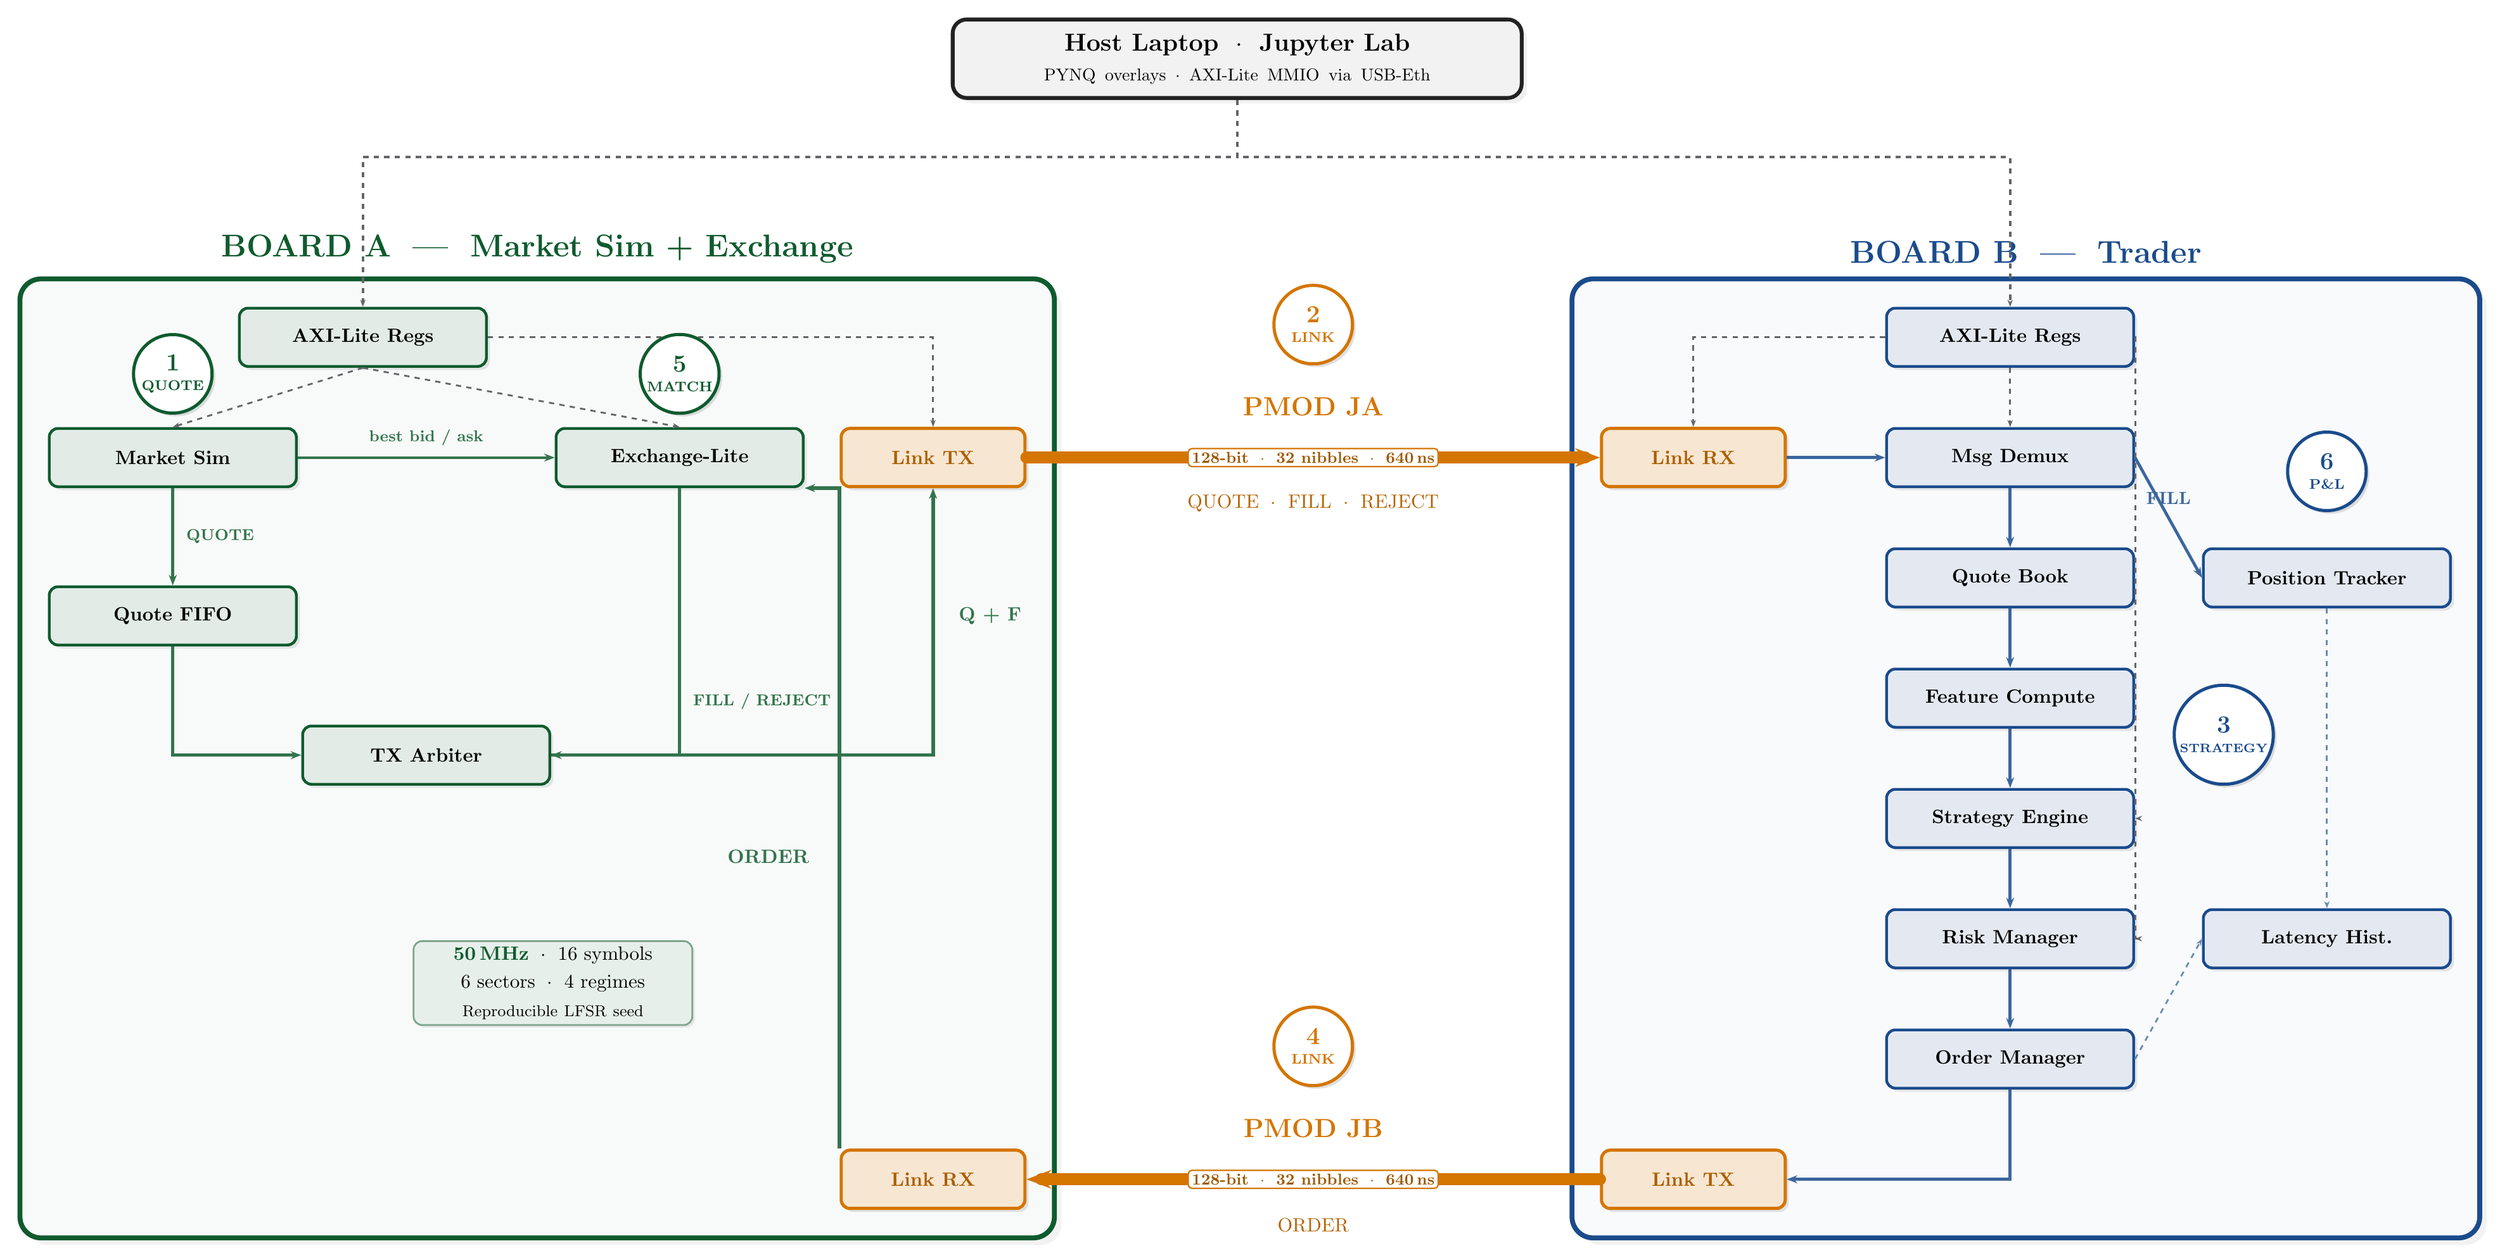
\begin{tikzpicture}[
  x=1in, y=1in,
  >=Stealth,
  every node/.style={font=\fontsize{12}{15}\selectfont},
  block/.style={
    rectangle, rounded corners=5pt, draw=#1, line width=1.6pt,
    fill=#1!12, minimum height=0.46in, minimum width=1.95in,
    align=center, font=\fontsize{11}{14}\selectfont\bfseries,
    inner sep=2pt,
    drop shadow={shadow xshift=2pt, shadow yshift=-2pt, opacity=0.18}
  },
  smallblock/.style={
    rectangle, rounded corners=5pt, draw=#1, line width=1.6pt,
    fill=#1!18, minimum height=0.46in, minimum width=1.45in,
    align=center, font=\fontsize{11}{14}\selectfont\bfseries,
    inner sep=2pt,
    drop shadow={shadow xshift=2pt, shadow yshift=-2pt, opacity=0.18}
  },
  linkblock/.style={
    rectangle, rounded corners=5pt, draw=linkcolor, line width=1.8pt,
    fill=linkcolor!18, minimum height=0.46in, minimum width=1.45in,
    align=center, font=\fontsize{11}{14}\selectfont\bfseries\color{linkcolor!80!black},
    inner sep=2pt,
    drop shadow={shadow xshift=2pt, shadow yshift=-2pt, opacity=0.20}
  },
  bigbox/.style={
    rectangle, rounded corners=12pt, draw=#1, line width=2.8pt,
    fill=#1!3, inner sep=0.22in,
    drop shadow={shadow xshift=4pt, shadow yshift=-4pt, opacity=0.10}
  },
  flow/.style={line width=1.7pt, color=#1!85, -{Stealth[length=6pt]}},
  axi/.style ={line width=1.0pt, color=uwgray, dashed, -{Stealth[length=4pt]}},
  cable/.style={line width=7pt, color=linkcolor, -{Stealth[length=14pt]},
                line cap=round},
  stagecirc/.style={
    circle, draw=#1, line width=1.8pt, fill=white, inner sep=1pt,
    minimum size=0.62in, align=center,
    font=\bfseries\color{#1},
    drop shadow={shadow xshift=1.8pt, shadow yshift=-1.8pt, opacity=0.25}
  },
  frametag/.style={
    rectangle, rounded corners=2pt, draw=linkcolor, line width=0.8pt,
    fill=white, inner sep=2pt,
    font=\fontsize{9}{11}\selectfont\bfseries\color{linkcolor!75!black}
  },
]

% =========================== HOST =====================================
% Compact, slightly left of center so Board B's heading has clear space.
\node[rectangle, rounded corners=8pt, draw=uwdark, line width=2.2pt,
      fill=uwlightgray, minimum height=0.62in, text width=4.4in,
      align=center, font=\fontsize{14}{18}\selectfont\bfseries,
      drop shadow={shadow xshift=3pt, shadow yshift=-3pt, opacity=0.12}]
  (host) at (-0.6, 0.20)
  {Host Laptop \;$\cdot$\; Jupyter Lab\\[-1pt]
   {\fontsize{10}{13}\selectfont\normalfont
    PYNQ overlays \(\cdot\) AXI-Lite MMIO via USB-Eth}};

% ===== LAYOUT GRID ==========================================================
%
%  Board A (7 visible modules from board_a_top.sv):
%    columns:  left=-9.0   center=-7.5   right=-5.0   link=-3.0
%    rows:     AXI=-2.0    row2=-2.95   QFIFO=-4.20  TXArb=-5.30
%              spec=-7.10  LinkRX=-8.65
%
%  Board B (11 visible modules from board_b_top.sv):
%    columns:  link=3.0    pipeline=5.5   side=7.5
%    rows:     AXI=-2.0    row2=-2.95   stride 0.95 down to OMgr=-7.70
%              LinkTX=-8.65
%
%  Cable alignment (perfectly horizontal):
%    A.LinkTX (y=-2.95)  <-->  B.LinkRX (y=-2.95)        PMOD JA
%    A.LinkRX (y=-8.65)  <-->  B.LinkTX (y=-8.65)        PMOD JB
%
%  Q+F  arrow rises at  x = -3.0  (LinkTX/LinkRX column centerline)
%  ORDER arrow rises at x = -3.85 (just LEFT of link column, no collision)
%
% ============================================================================

% =========================== BOARD B (right) ================================
\node[block=boardBcolor]   (b_axi)    at ( 5.5, -2.0)  {AXI-Lite Regs};
\node[linkblock]           (b_linkrx) at ( 3.0, -2.95) {Link RX};
\node[block=boardBcolor]   (b_demux)  at ( 5.5, -2.95) {Msg Demux};
\node[block=boardBcolor]   (b_qbook)  at ( 5.5, -3.90) {Quote Book};
\node[block=boardBcolor]   (b_feat)   at ( 5.5, -4.85) {Feature Compute};
\node[block=boardBcolor]   (b_strat)  at ( 5.5, -5.80) {Strategy Engine};
\node[block=boardBcolor]   (b_risk)   at ( 5.5, -6.75) {Risk Manager};
\node[block=boardBcolor]   (b_omgr)   at ( 5.5, -7.70) {Order Manager};
\node[linkblock]           (b_linktx) at ( 3.0, -8.65) {Link TX};
\node[block=boardBcolor]   (b_pos)    at ( 8.0, -3.90) {Position Tracker};
\node[block=boardBcolor]   (b_lat)    at ( 8.0, -6.75) {Latency Hist.};

\begin{scope}[on background layer]
  \node[bigbox=boardBcolor,
        fit=(b_axi)(b_linkrx)(b_demux)(b_qbook)(b_feat)(b_strat)
            (b_risk)(b_omgr)(b_linktx)(b_pos)(b_lat),
        label={[font=\fontsize{18}{22}\selectfont\bfseries
               \color{boardBcolor}, yshift=0.06in]above:%
               BOARD B \;\textemdash\; Trader}
  ] (boxB) {};
\end{scope}

% Board B AXI fan-out (config plane, dashed)
\draw[axi] (b_axi.south) -- (b_demux.north);
\draw[axi] (b_axi.west)  -| (b_linkrx.north);
\draw[axi] (b_axi.east)  -| ([xshift=0.30]b_strat.east) -- (b_strat.east);
\draw[axi] (b_axi.east)  -| ([xshift=0.30]b_risk.east)  -- (b_risk.east);

% Pipeline data flow (vertical: top -> bottom)
\draw[flow=boardBcolor] (b_linkrx.east) -- (b_demux.west);
\draw[flow=boardBcolor] (b_demux)  -- (b_qbook);
\draw[flow=boardBcolor] (b_qbook)  -- (b_feat);
\draw[flow=boardBcolor] (b_feat)   -- (b_strat);
\draw[flow=boardBcolor] (b_strat)  -- (b_risk);
\draw[flow=boardBcolor] (b_risk)   -- (b_omgr);
\draw[flow=boardBcolor] (b_omgr.south) |- (b_linktx.east);

% Side branch: Demux -> Position Tracker (FILL feedback)
\draw[flow=boardBcolor] (b_demux.east) -- (b_pos.west)
  node[midway, above=0.05,
       font=\fontsize{10}{12}\selectfont\bfseries\color{boardBcolor!85}]{FILL};

% Latency-histogram timing taps (very thin, dotted -- it's instrumentation)
\draw[axi, color=boardBcolor!65, line width=1.0pt]
  (b_omgr.east) -- (b_lat.west);
\draw[axi, color=boardBcolor!65, line width=1.0pt]
  (b_pos.south) -- (b_lat.north);

% =========================== BOARD A (left) =================================
\node[block=boardAcolor]   (a_axi)    at (-7.5, -2.0)  {AXI-Lite Regs};
\node[block=boardAcolor]   (a_msim)   at (-9.0, -2.95) {Market Sim};
\node[block=boardAcolor]   (a_exch)   at (-5.0, -2.95) {Exchange-Lite};
\node[linkblock]           (a_linktx) at (-3.0, -2.95) {Link TX};
\node[block=boardAcolor]   (a_qfifo)  at (-9.0, -4.20) {Quote FIFO};
\node[block=boardAcolor]   (a_txarb)  at (-7.0, -5.30) {TX Arbiter};
\node[linkblock]           (a_linkrx) at (-3.0, -8.65) {Link RX};

\begin{scope}[on background layer]
  \node[bigbox=boardAcolor,
        fit=(a_axi)(a_msim)(a_exch)(a_qfifo)(a_txarb)(a_linktx)(a_linkrx),
        label={[font=\fontsize{18}{22}\selectfont\bfseries
               \color{boardAcolor}, yshift=0.06in]above:%
               BOARD A \;\textemdash\; Market Sim + Exchange}
  ] (boxA) {};
\end{scope}

% --- Board A AXI config (dashed) ---
\draw[axi] (a_axi.south) -- (a_msim.north);
\draw[axi] (a_axi.south) -- (a_exch.north);
\draw[axi] (a_axi.east)  -| (a_linktx.north);

% --- Board A data plane ---
% (1) Market Sim continuously feeds Exchange with best bid/ask
\draw[flow=boardAcolor, line width=1.4pt]
   (a_msim.east) -- (a_exch.west)
   node[midway, above=0.04,
        font=\fontsize{9}{11}\selectfont\bfseries\color{boardAcolor!85}]
        {best bid / ask};

% (2) Market Sim -> Quote FIFO -> TX Arbiter (quote stream)
\draw[flow=boardAcolor] (a_msim.south) -- (a_qfifo.north)
   node[midway, right=0.05,
        font=\fontsize{9}{11}\selectfont\bfseries\color{boardAcolor!85}]
        {QUOTE};
\draw[flow=boardAcolor] (a_qfifo.south) |- (a_txarb.west);

% (3) Exchange-Lite -> TX Arbiter (fill / reject)
\draw[flow=boardAcolor] (a_exch.south) |- (a_txarb.east)
   node[pos=0.40, right=0.05,
        font=\fontsize{9}{11}\selectfont\bfseries\color{boardAcolor!85}]
        {FILL / REJECT};

% (4) TX Arbiter -> Link TX  -- arrow rises at x = -3.0
\draw[flow=boardAcolor, line width=2.0pt]
   (a_txarb.east) -| (a_linktx.south);
\node[font=\fontsize{11}{14}\selectfont\bfseries\color{boardAcolor!85}]
   at (-2.55, -4.20) {Q + F};

% (5) Link RX -> Exchange  -- arrow rises at x = -3.85 (clear of Link column)
\draw[flow=boardAcolor, line width=2.0pt]
   ([xshift=-0.125]a_linkrx.north west) |- (a_exch.south east);
\node[font=\fontsize{11}{14}\selectfont\bfseries\color{boardAcolor!85}]
   at (-4.30, -6.10) {ORDER};

% --- Board A: spec badge fills the central empty area ---
\node[rectangle, rounded corners=5pt, fill=boardAcolor!10,
      draw=boardAcolor!55, line width=1.0pt,
      minimum width=2.20in, text width=2.05in,
      align=center, font=\fontsize{11}{14}\selectfont,
      anchor=center,
      drop shadow={shadow xshift=1.5pt, shadow yshift=-1.5pt, opacity=0.15}]
  (a_specs) at (-6.0, -7.10)
  {\textbf{\color{boardAcolor}50\,MHz} \;$\cdot$\; 16 symbols\\[2pt]
   6 sectors \;$\cdot$\; 4 regimes\\[2pt]
   {\fontsize{9}{11}\selectfont
    Reproducible LFSR seed}};

% =========================== HOST AXI =======================================
\draw[axi, line width=1.5pt] (host.south) -- ++(0,-0.45) -| (a_axi.north);
\draw[axi, line width=1.5pt] (host.south) -- ++(0,-0.45) -| (b_axi.north);

% =========================== PMOD CABLES (thick + frame tags) ==============
%   Each cable runs in its own dedicated horizontal "lane" -- no overlap.
% PMOD JA  (top, A->B):  Quote / Fill / Reject
\draw[cable] (a_linktx.east) -- (b_linkrx.west);
\node[font=\fontsize{15}{18}\selectfont\bfseries\color{linkcolor}]
  at ($(a_linktx.east)!0.5!(b_linkrx.west) + (0,0.40)$) {PMOD JA};
\node[frametag]
  at ($(a_linktx.east)!0.5!(b_linkrx.west)$)
  {128-bit \;$\cdot$\; 32 nibbles \;$\cdot$\; 640\,ns};
\node[font=\fontsize{11}{14}\selectfont\color{linkcolor!85!black}]
  at ($(a_linktx.east)!0.5!(b_linkrx.west) + (0,-0.36)$)
  {QUOTE \;$\cdot$\; FILL \;$\cdot$\; REJECT};

% PMOD JB  (bottom, B->A):  Order
\draw[cable] (b_linktx.west) -- (a_linkrx.east);
\node[font=\fontsize{15}{18}\selectfont\bfseries\color{linkcolor}]
  at ($(b_linktx.west)!0.5!(a_linkrx.east) + (0,0.40)$) {PMOD JB};
\node[frametag]
  at ($(b_linktx.west)!0.5!(a_linkrx.east)$)
  {128-bit \;$\cdot$\; 32 nibbles \;$\cdot$\; 640\,ns};
\node[font=\fontsize{11}{14}\selectfont\color{linkcolor!85!black}]
  at ($(b_linktx.west)!0.5!(a_linkrx.east) + (0,-0.36)$) {ORDER};

% =========================== STAGE BADGES ==================================
% Each stage circle now contains BOTH a number and the action it represents,
% so the round-trip flow (1) Quote -> (2) Link -> (3) Strategy -> (4) Link
% -> (5) Match -> (6) P&L is self-documenting on the diagram.
\node[stagecirc=boardAcolor] at ($(a_msim.north)        +(0,0.42)$)
   {\fontsize{14}{14}\selectfont 1\\[-1pt]
    {\fontsize{8}{9}\selectfont QUOTE}};
\node[stagecirc=linkcolor]   at ($(a_linktx.east)!0.5!(b_linkrx.west)
                                  +(0,1.05)$)
   {\fontsize{14}{14}\selectfont 2\\[-1pt]
    {\fontsize{8}{9}\selectfont LINK}};
\node[stagecirc=boardBcolor] at ($(b_strat.north east)  +(0.70,0.42)$)
   {\fontsize{14}{14}\selectfont 3\\[-1pt]
    {\fontsize{7}{8}\selectfont STRATEGY}};
\node[stagecirc=linkcolor]   at ($(b_linktx.west)!0.5!(a_linkrx.east)
                                  +(0,1.05)$)
   {\fontsize{14}{14}\selectfont 4\\[-1pt]
    {\fontsize{8}{9}\selectfont LINK}};
\node[stagecirc=boardAcolor] at ($(a_exch.north)        +(0,0.42)$)
   {\fontsize{14}{14}\selectfont 5\\[-1pt]
    {\fontsize{8}{9}\selectfont MATCH}};
\node[stagecirc=boardBcolor] at ($(b_pos.north)         +(0,0.60)$)
   {\fontsize{14}{14}\selectfont 6\\[-1pt]
    {\fontsize{8}{9}\selectfont P\&L}};

\end{tikzpicture}
\end{center}%
}

\vspace{0.50in}

% ===========================================================================
%  ROW 2.5 - THE MATH BEHIND THE PIPELINE (full width, compact 4-col)
% ===========================================================================
\sectionbox{uwdark}{The Math Behind the Pipeline}{%
\vspace{-0.05in}
Every quantity is \textbf{fixed-point}, every op is \textbf{shift-and-add},
every stage has a \textbf{deterministic cycle cost} --- the discipline that
makes hardware trading cycle-accurate.

\vspace{0.12in}

\begin{minipage}[t]{8.0in}
{\fontsize{18}{22}\selectfont\bfseries\color{boardAcolor}%
 1.\;Fixed-Point}

\vspace{0.04in}
{\fontsize{14}{18}\selectfont\itshape\color{uwgray}%
 Why every number is integer-encoded and why that gives us zero jitter.}

\vspace{0.06in}
Floats add unpredictable rounding. We use two scaled-integer
formats so the FPGA does ordinary integer adds:
\begin{itemize}[leftmargin=0.24in, itemsep=0.03in, labelsep=0.08in,
                topsep=0.04in]
  \item[\color{boardAcolor}\textbullet]
    \textbf{Q16.16} (u32) for prices, spreads, EMAs ---
    16 integer bits ($\$0$--$\$65{,}535$), 16 fraction bits
    ($\sim\!\$1.5\!\!\times\!\!10^{-5}$ resolution)
  \item[\color{boardAcolor}\textbullet]
    \textbf{Q32.16} (s48) for cash and P\&L ---
    handles \(\pm\$2.1\)\,B before saturation
  \item[\color{boardAcolor}\textbullet]
    \textbf{1-cycle} add/sub everywhere; no FPU \(\Rightarrow\)
    no NaN/Inf, \textbf{zero jitter} between identical runs
  \item[\color{boardAcolor}\textbullet]
    Same LFSR seed \(\Rightarrow\) bit-exact replays for debug
\end{itemize}
\end{minipage}\hfill
\begin{minipage}[t]{8.0in}
{\fontsize{18}{22}\selectfont\bfseries\color{boardAcolor}%
 2.\;Market Sim (A)}

\vspace{0.04in}
{\fontsize{14}{18}\selectfont\itshape\color{uwgray}%
 How 16 stock prices wander realistically without ever drifting away.}

\vspace{0.06in}
Each tick, a price is pulled toward its anchor (mean-reversion)
plus three layers of random shock:
\[
  p_{s,t+1} = p_{s,t}
   + \underbrace{\kappa_r(\bar{p}_s - p_{s,t})}_{\text{pull to anchor}}
   + \underbrace{\sigma_r(n_{g}+n_{\mathrm{sec}}+n_s)}_{\text{3-tier noise}}
\]
\(\kappa_r,\sigma_r\) flip with the regime ---
\textbf{CALM}\,\(\to\)\,\textbf{VOL}\,\(\to\)\,\textbf{BURST}\,\(\to\)\,\textbf{ADV}.
Three LFSR-32s (period \(2^{32}\!-\!1\)) feed the noise.
Bid/ask = \(p_s\!\pm\!\tfrac{1}{2}\mathrm{spread}_s\).
\end{minipage}\hfill
\begin{minipage}[t]{8.0in}
{\fontsize{18}{22}\selectfont\bfseries\color{boardBcolor}%
 3.\;Strategy + Risk (B)}

\vspace{0.04in}
{\fontsize{14}{18}\selectfont\itshape\color{uwgray}%
 ``Cheap reverts up, rich reverts down,'' with 3 safety nets.}

\vspace{0.06in}
\textbf{1.\;Fair value} (single-DSP EMA --- a smoothed estimate of the
``true'' price):\;
\(\mu_{s,t+1}\!=\!\mu_{s,t}\!+\!\alpha(p_{s,t}\!-\!\mu_{s,t})\)

\smallskip
\textbf{2.\;Decision} ($\Delta\!=\!$ how far above/below fair value;
threshold \(\theta\) replaces division by \(\sigma\)):\;
\(\Delta_s\!=\!p_s\!-\!\mu_s\;\Rightarrow\;\)\textcolor{boardBcolor!85}{BUY}
if cheap, \textcolor{boardBcolor!85}{SELL} if rich.

\smallskip
\textbf{3.\;Safety} (3 parallel comparators block bad orders):\;
position \(|q_s\!+\!\delta|\!\le\!Q_{\max}\), rate
\(r_t\!\le\!r_{\max}\), drawdown \(C_t\!\ge\!-L_{\max}\).

\smallskip
\textbf{4.\;P\&L} (after every accepted FILL):\;
\(\mathrm{P\&L}_t = C_t + \sum_{s} q_s\,p_s\)
\end{minipage}\hfill
\begin{minipage}[t]{8.0in}
{\fontsize{18}{22}\selectfont\bfseries\color{linkcolor}%
 4.\;Latency}

\vspace{0.04in}
{\fontsize{14}{18}\selectfont\itshape\color{uwgray}%
 Why we can quote a single number and trust it.}

\vspace{0.06in}
Every stage has a fixed cycle count, so the round-trip is just
their sum (no OS, no contention):
\[
  T_{\mathrm{RT}} =
  \underbrace{1}_{\text{quote}} +
  \underbrace{32}_{\text{A}\to\text{B}} +
  \underbrace{6}_{\text{pipe}} +
  \underbrace{32}_{\text{B}\to\text{A}} +
  \underbrace{1}_{\text{match}}\;\text{cy}
\]
\(@\,50\,\mathrm{MHz}\;(20\,\mathrm{ns/cy})\):\;
\(T_{\mathrm{RT}}\!\approx\!72\,\mathrm{cy}\!=\!\mathbf{1.44\,\mu s}\),
\textbf{every quote, no exceptions}. The on-chip Latency Histogram
(\(16\!\times\!8\)\,cy bins) measures
\(\Delta t = t_{\mathrm{fill}}\!-\!t_{\mathrm{send}}\) in fabric, so
the metric itself is jitter-free.
\end{minipage}
}

\vspace{0.50in}

% ===========================================================================
%  ROW 3 - HARDWARE IMPLEMENTATION (full width, 3 columns: A | link | B)
% ===========================================================================
\sectionbox{uwdark}{Hardware Implementation}{%
\vspace{-0.05in}
Two AMD Zynq UltraScale+ \textbf{XCZU3EG} boards, all logic written
in SystemVerilog around a shared \texttt{hft\_pkg.sv}, every
register-mapped surface driven from Python over AXI-Lite MMIO.

\vspace{0.18in}

% ---- Column 1: Board A ----------------------------------------------------
\begin{minipage}[t]{10.6in}
{\fontsize{22}{26}\selectfont\bfseries\color{boardAcolor}%
 Board A \;\textemdash\; Market Sim + Exchange}

\vspace{0.06in}
{\fontsize{14}{18}\selectfont\itshape\color{uwgray}%
 Generates 16 correlated stock prices and matches incoming orders
 against best bid/ask in 1 cycle.}

\vspace{0.10in}
\begin{itemize}[leftmargin=0.30in, itemsep=0.06in, labelsep=0.10in]
  \item[\color{boardAcolor}\textbullet]
    \textbf{Market Sim:} 3-tier LFSR noise (global / sector /
    per-symbol) with O--U pull-back; 4 regimes (CALM\,$\to$\,VOL\,$\to$\,BURST\,$\to$\,ADV)
  \item[\color{boardAcolor}\textbullet]
    \textbf{Quote FIFO + TX Arbiter:} buffers quotes, prioritizes
    fill/reject responses for fair link bandwidth
  \item[\color{boardAcolor}\textbullet]
    \textbf{Exchange-Lite:} 1-cycle order match against live best
    bid/ask; emits \textsc{FILL} or \textsc{REJECT}
  \item[\color{boardAcolor}\textbullet]
    \textbf{AXI-Lite regs:} per-symbol mid, spread, sector, 16-bit
    company tokens --- all writable live from Python
\end{itemize}

\vspace{0.10in}
{\fontsize{13}{17}\selectfont\color{uwdark}%
\textbf{FSM:}\; RESET\,$\to$\,IDLE\,$\to$\,RUNNING\,$\leftrightarrow$\,STOPPED}
\end{minipage}\hfill
% ---- Column 2: Link Layer -------------------------------------------------
\begin{minipage}[t]{10.6in}
{\fontsize{22}{26}\selectfont\bfseries\color{linkcolor}%
 Link Layer \;\textemdash\; Custom PMOD}

\vspace{0.06in}
{\fontsize{14}{18}\selectfont\itshape\color{uwgray}%
 Full-duplex 128-bit framed bus over two PMOD ribbons --- our own
 protocol, no IP-core black boxes.}

\vspace{0.10in}
\begin{itemize}[leftmargin=0.30in, itemsep=0.06in, labelsep=0.10in]
  \item[\color{linkcolor}\textbullet]
    \textbf{Physical:} 2$\times$12-pin PMOD (JA: A$\to$B,\; JB: B$\to$A)
    --- simultaneous quote and order paths
  \item[\color{linkcolor}\textbullet]
    \textbf{Frame:} 128 b = 4-b msg\_type + 4-b sym\_id + 32-b bid +
    32-b ask + 16-b qty + 16-b seq + 24-b rsvd/CRC
  \item[\color{linkcolor}\textbullet]
    \textbf{Mesochronous CDC:} each board has its own crystal;
    2-FF synchronizer at every RX nibble deserializer
  \item[\color{linkcolor}\textbullet]
    \textbf{Throughput:} 32 nibbles\,$\times$\,20\,ns = \textbf{640\,ns/frame};
    1.5\,M frames/s ceiling, 64-deep TX FIFOs absorb burst storms
\end{itemize}

\vspace{0.10in}
{\fontsize{13}{17}\selectfont\color{uwdark}%
\textbf{Handshake:}\; ready/valid on both ends, no dropped frames}
\end{minipage}\hfill
% ---- Column 3: Board B ----------------------------------------------------
\begin{minipage}[t]{10.6in}
{\fontsize{22}{26}\selectfont\bfseries\color{boardBcolor}%
 Board B \;\textemdash\; Trader Pipeline}

\vspace{0.06in}
{\fontsize{14}{18}\selectfont\itshape\color{uwgray}%
 7-stage deterministic pipeline; one quote in $\to$ one order out, in
 a fixed cycle count every time.}

\vspace{0.10in}
\begin{itemize}[leftmargin=0.30in, itemsep=0.06in, labelsep=0.10in]
  \item[\color{boardBcolor}\textbullet]
    \textbf{Demux + Quote Book:} routes by msg\_type, maintains live
    best bid/ask for all 16 symbols
  \item[\color{boardBcolor}\textbullet]
    \textbf{Feature Compute:} single-DSP per-symbol EMA fair value,
    deviation $\Delta = p_s - \mu_s$
  \item[\color{boardBcolor}\textbullet]
    \textbf{Strategy + Risk:} Mean-Rev (default) / Momentum / NN-stub
    / Auto; 3 parallel comparators for position, rate, drawdown caps
  \item[\color{boardBcolor}\textbullet]
    \textbf{Position Tracker + Latency Hist:} Q32.16 cash + per-symbol
    qty; on-chip 16-bin quote-to-fill measurement
\end{itemize}

\vspace{0.10in}
{\fontsize{13}{17}\selectfont\color{uwdark}%
\textbf{FSM:}\; B\_RESET\,$\to$\,B\_IDLE\,$\to$\,B\_ARMED\,$\to$\,B\_TRADING\,$\leftrightarrow$\,B\_HALTED}
\end{minipage}
}

\vspace{0.22in}

% ===========================================================================
%  ROW 5 - CONCLUSIONS & KEY PERFORMANCE
%   Top: 3 headline metric cards.
%   Bottom: 2-col takeaway bullets (one bullet = how we verified).
% ===========================================================================
\begin{center}
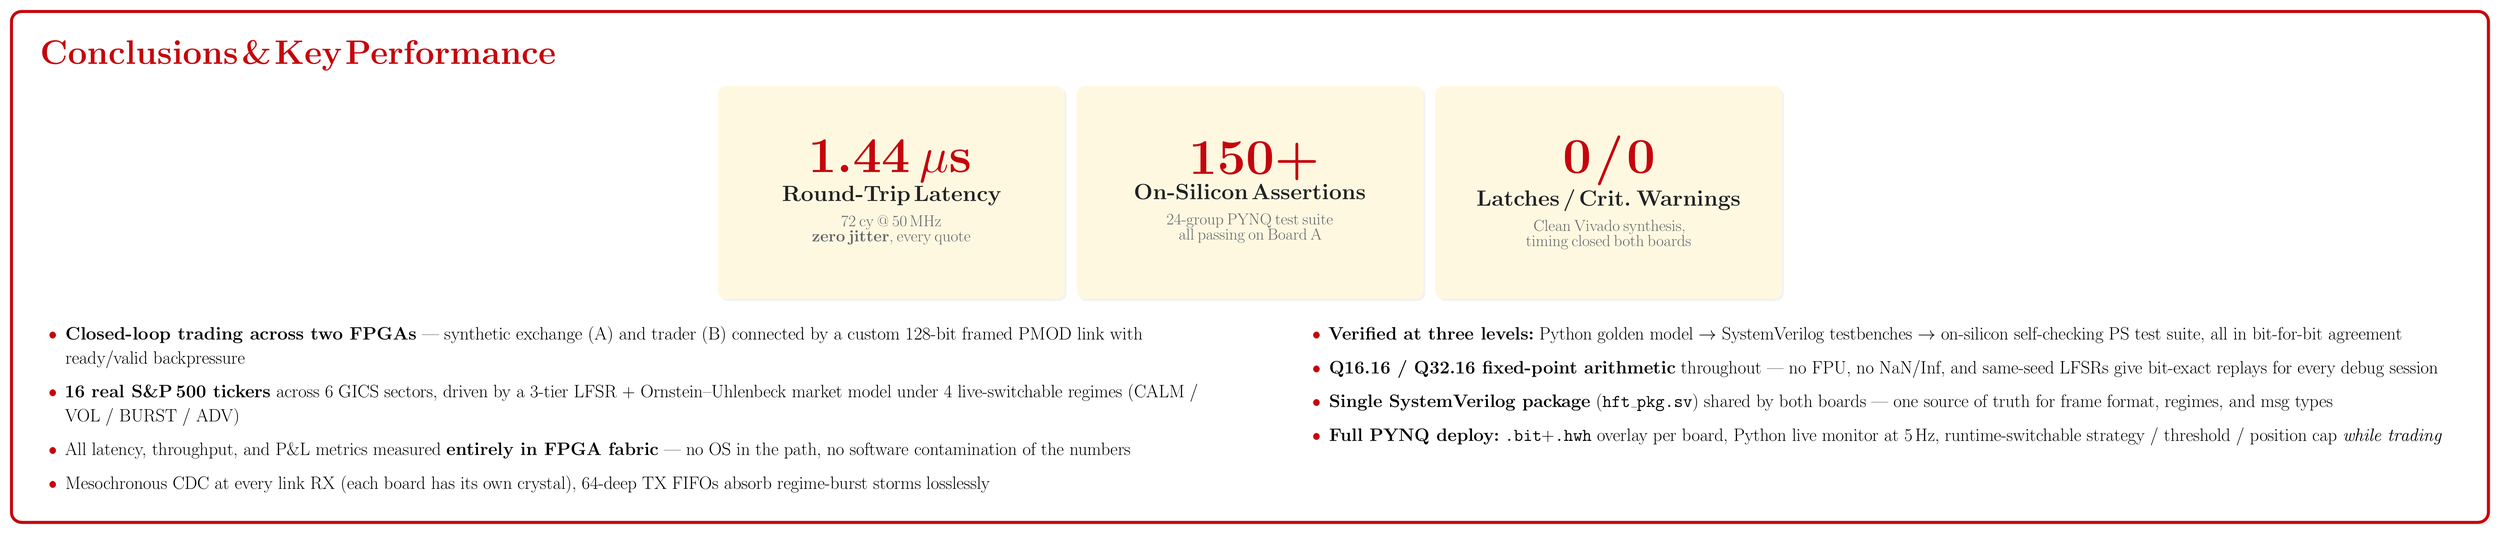
\begin{tikzpicture}
\node[
  inner sep=0.40in,
  fill=white,
  rounded corners=10pt,
  draw=uwred, line width=3pt,
  text width=33.5in,
  align=left,
  drop shadow={shadow xshift=3pt, shadow yshift=-3pt, opacity=0.12}
] {%
  {\fontsize{34}{40}\selectfont\bfseries\color{uwred}
    Conclusions \& Key Performance}\\[0.20in]

  % ---- METRIC ROW (3 cards) ----------------------------------------------
  \begin{center}
  \begin{tabular}{@{}c c c@{}}
  \metriccard{1.44\,$\mu$s}{Round-Trip Latency}{%
  72 cy @ 50\,MHz\\
  \textbf{zero jitter}, every quote}
  &
  \metriccard{150+}{On-Silicon Assertions}{%
  24-group PYNQ test suite\\
  all passing on Board A}
  &
  \metriccard{0 / 0}{Latches / Crit. Warnings}{%
  Clean Vivado synthesis,\\
  timing closed both boards}
  \end{tabular}
  \end{center}

  \vspace{0.18in}

  {\fontsize{18}{24}\selectfont\RaggedRight

  \begin{minipage}[t]{16.0in}
  \begin{itemize}[leftmargin=0.35in, itemsep=0.08in, labelsep=0.12in]
    \item[\color{uwred}\textbullet]
      \textbf{Closed-loop trading across two FPGAs} ---
      synthetic exchange (A) and trader (B) connected by a custom
      128-bit framed PMOD link with ready/valid backpressure
    \item[\color{uwred}\textbullet]
      \textbf{16 real S\&P\,500 tickers} across 6 GICS sectors,
      driven by a 3-tier LFSR + Ornstein--Uhlenbeck market model
      under 4 live-switchable regimes (CALM / VOL / BURST / ADV)
    \item[\color{uwred}\textbullet]
      All latency, throughput, and P\&L metrics measured
      \textbf{entirely in FPGA fabric} --- no OS in the path,
      no software contamination of the numbers
    \item[\color{uwred}\textbullet]
      Mesochronous CDC at every link RX (each board has its own
      crystal), 64-deep TX FIFOs absorb regime-burst storms losslessly
  \end{itemize}
  \end{minipage}\hfill
  \begin{minipage}[t]{16.0in}
  \begin{itemize}[leftmargin=0.35in, itemsep=0.08in, labelsep=0.12in]
    \item[\color{uwred}\textbullet]
      \textbf{Verified at three levels:} Python golden model
      $\to$ SystemVerilog testbenches $\to$ on-silicon self-checking
      PS test suite, all in bit-for-bit agreement
    \item[\color{uwred}\textbullet]
      \textbf{Q16.16 / Q32.16 fixed-point arithmetic} throughout ---
      no FPU, no NaN/Inf, and same-seed LFSRs give bit-exact replays
      for every debug session
    \item[\color{uwred}\textbullet]
      \textbf{Single SystemVerilog package} (\texttt{hft\_pkg.sv})
      shared by both boards --- one source of truth for frame format,
      regimes, and msg types
    \item[\color{uwred}\textbullet]
      \textbf{Full PYNQ deploy:} \texttt{.bit}+\texttt{.hwh} overlay
      per board, Python live monitor at 5\,Hz, runtime-switchable
      strategy / threshold / position cap \emph{while trading}
  \end{itemize}
  \end{minipage}

  }%
};
\end{tikzpicture}
\end{center}

\end{minipage}

\end{document}
